\documentclass{article}
\usepackage[utf8]{inputenc}
\usepackage[russian]{babel}
%\usepackage{systeme}
\usepackage{amsmath}
\usepackage{amssymb}
\usepackage{amsfonts}
\usepackage{mathtext}


%\usepackage[dvips]{graphicx}
\usepackage[final]{graphicx}
\graphicspath{{noiseimages/}}

\renewcommand{\baselinestretch}{1.5}

\title{Третье задание по БМСО}
\author{Ярослав Аверьянов}
\date{Октябрь 2015}

\begin{document}

\maketitle

\section{Первая задача}
\begin{center} 
$||P - Q||_{TV} = 2\cdot \underset{B \in \mathbf{B}}{sup}|P(B) - Q(B)|$ - общая дисперсия $P$ и $Q$.
\end{center}
Для непрерывных распределений $P$ и $Q$ с плотностями $p$ и $q$ обозначим
\begin{center}
$||P - Q||_d = \int |p - q|d\mu$
\end{center}
Докажем эквивалентность $||\cdot||_{TV}$ и $||\cdot||_d$ для непрерывных распределений.\\
Пусть $A = [x|p(x) - q(x) \leq 0] \in \mathbf{B}$ - замкнутое и измеримое множество.\\
Пусть $B \in \mathbf{B}$:\\
$P(B) - Q(B) = \int_{B} (p(x) - q(x))dx = \int_A (p(x) - q(x))dx + \int_{B \ A} (p(x) - q(x))dx - \int_{A \ B} (p(x) - q(x))dx$\\
Где $\int_{B \ A} (p(x) - q(x))dx \leq 0, \int_{A \ B} (p(x) - q(x))dx \geq 0$
$\to P(B) - Q(B) \leq \int_A (p(x) - q(x))dx = P(A) - Q(A)$\\
$Для \overline{A} = {x|p(x) - q(x) \geq 0}$:\\
$Q(B) - P(B) \leq Q(\overline{A}) - P(\overline{A}) = P(A) - Q(A)$.\\
Поэтому $|P(B) - Q(B)| \leq P(A) - Q(A)$.
$\to ||P - Q||_{TV} = 2\cdot \underset{B \in \mathbf{B}}{sup}|P(B) - Q(B)| = 2\cdot(P(A) - Q(A)) = P(A) - Q(A) - (1 - P(A)) + (1 - Q(A)) = \int_A (p - q)d\mu + \int_{\overline{A}} (p - q)d\mu = ||p - q||_{d}$.

\section{Вторая задача}
Пусть $X \sim N(\mu_1, \sigma_1^2), Y \sim N(\mu_2, \sigma_2^2).$ Используя то, что $d_{TV}(X, Y) = \frac{1}{2}\int_{-\infty}^{+\infty} |f(x) - g(x)|dx$, где $f$ и $g$ - плотности для $X$ и $Y$. Далее предположим, что $\sigma_1 > \sigma_2$.\\
Введем следующие обозначения:
\begin{center}
$c = \frac{\sigma_1}{\sigma_2} \qquad \Delta = \frac{\mu_1 - \mu_2}{\sigma_2}$\\
$A = \frac{\sqrt{(c^2 - 1)2log(c) + \Delta^2} - c\Delta}{c^2 - 1}, \qquad B = -\frac{\sqrt{(c^2 - 1)2log(c) + \Delta^2} + c\Delta}{c^2 - 1}$
\end{center}
Используя эти обозначения:
\begin{center}
$\int_{-\infty}^{+\infty} |f(x) - g(x)|dx = \int_{-\infty}^{+\infty} |\phi(z) - c\phi(\Delta + cz)|dz$
\end{center}
И $\phi(z) \leq c\phi(\Delta + cz) <-> A \leq z \leq B$. Следовательно\\
$\int_{-\infty}^{+\infty}|f(x) - g(x)|dx = \int_A^B [c\phi(\Delta + cz) - \phi(z)]dz + \int_{-\infty}^A [\phi(z) - c\phi(\Delta + cz)]dz + \int_B^{+\infty}[\phi(z) - c\phi(\Delta + cz)]dz = 2[(\Phi(\Delta + cB) - \Phi(B)) - (\Phi(\Delta + cA) - \Phi(A))].$\\
Где 
\begin{center}
$\Delta + cB = \frac{c\sqrt{(c^2 - 1)2log(c) + \Delta^2} - \Delta}{c^2 - 1}$\\
$\Delta + cA = -\frac{c\sqrt{(c^2 - 1)2log(c) + \Delta^2} + \Delta}{c^2 - 1}$
\end{center}
Если $\sigma_1 = \sigma_2$, формула сокращается до $\Phi(\frac{|\Delta|}{2}) - \Phi(-\frac{|\Delta|}{2})$\\
Следовательно, $d_{TV}(X,Y) = (\Phi(\Delta + cB) - \Phi(B)) - (\Phi(\Delta + cA) - \Phi(A))$

\section{Третья задача}
Показать, что если:\\
У1) множество параметров $\theta \in \Theta \subset \mathbf{R}$ - ограниченное открытое множество.\\
У2) $\exists \sigma > 0 : \forall \theta \in \Theta$ информация Фишера $I(\theta)$:
\begin{center}
$I(\theta) > \sigma > 0,$
\end{center}
то для экспоненциального семейства распределений выполнено "предположение (5)" теоремы Бернштейна-фон-Мизеса.\\
Плотность распределения: $p(x|\theta) = exp(-c(\theta) + \theta t(x))$\\
$1 = \int exp(-c(\theta) + \theta t(x))dx, c(\theta) = ln \int exp(\theta t(x))dx$ - нормировка
\begin{center}
$c^{'}(\theta) = \frac{\int t(x)exp(\theta t(x))dx}{\int exp(\theta t(x))dx} = \int exp(-c(\theta) + \theta t(x))t(x)dx = \mathbf{E}_{\theta} t(x)$
\end{center}
Посчитаем информацию Фишера и логарифм правдоподобия:
\begin{center}
$I(\theta) = - \mathbf{E}[l^{''}(x|\theta)] = c^{''}(\theta) > \sigma > 0$\\
$L_n(\theta) = ln L(x_1,...,x_n|\theta) = -nc(\theta) + \theta \sum\limits_{i=1}^{n}t(x_i)$\\
$\frac{1}{n}(L_n(\theta) - L_n(\theta_0)) = c(\theta) - c(\theta_0) + \frac{1}{n}(\theta - \theta_0)\sum\limits_{i=1}^{n}t(x_i).$
\end{center}
Так как
\begin{center}
$c(\theta) - c(\theta_0) \geq (\theta - \theta_0)\mathbf{E}_{\theta}t(x) + \frac{\sigma}{2}(\theta - \theta_0)^2$
\end{center}
Получаем:
\begin{center}
$\frac{1}{n}(L_n(\theta) - L_n(\theta_0)) \leq (\theta - \theta_0)(-\mathbf{E}_{\theta}t(x) + \frac{1}{n}\sum\limits_{i=1}^n t(x_i)) - \frac{\sigma}{2}(\theta - \theta_0)^2$
\end{center}
Т.к. $\frac{1}{n}\sum\limits_{i=1}^n t(x_i) \overset{P}{\to} \mathbf{E}t(x), |\theta - \theta_0| < \gamma \to \forall \delta > 0 \exists \epsilon > 0 :$
\begin{center}
$P_{\theta_0}(\underset{|\theta - \theta_0 | < \delta}{sup}\frac{1}{n}(L_n(\theta) - L_n(\theta_0)) \leq -\epsilon) \geq P_{\theta_0}(\gamma|-\mathbf{E}t(x) + \frac{1}{n}\sum\limits_{i=1}^n t(x_i)| - \frac{\sigma}{2}\delta^2 < -\epsilon) = P_{\theta_0}(|-\mathbf{E}t(x) + \frac{1}{n}\sum\limits_{i=1}^n t(x_i)| < \frac{1}{\gamma}(\frac{\sigma}{2}\delta^2 - \epsilon)) \to 1,$ где $\epsilon < \frac{\sigma}{2}\delta^2$.
\end{center}

\section{Четвертая задача}
Получить оценку максимального правдоподобия $\hat{\theta_n}$ и байесовскую оценку $\theta_n^{*} = \int \theta p(\theta|x_1,...,x_n)d\theta$ для среденего $\mu$ нормального распределения $N(\mu,\sigma^2)$ и априорного распределения $\theta \sim N(\mu_{\text{П}}, \sigma_{\text{П}}^2)$.\\
Посчитаем правдоподобие:
\begin{center}
$L(x_1,...,x_n|\theta) = \frac{1}{(2\pi \sigma^2)^{\frac{n}{2}}} exp(-\frac{\sum\limits_{i=1}^n (x_i - \mu)^2}{2\sigma^2})$
\end{center}
Оценка максимального правдоподобия:
\begin{center}
$\hat{\mu_n} = \underset{\mu}{argmax}L(x_1,...,x_n|\mu) = \underset{\mu}{argmax}exp(-\frac{\sum\limits_{i=1}^n (x_i - \mu)^2}{2\sigma^2}) = \underset{\mu}{argmax}\sum\limits_{i=1}^n (x_i - \mu)^2 \to \hat{\mu_n} = \frac{1}{n}\sum\limits_{i=1}^n x_i.$
\end{center}
Байесовская оценка $\mu_n^{*} = \int \mu \cdot p(\mu|x_1,...,x_n)d\mu$\\
Априорное распределение $\mu \sim N(\mu_{\text{П}},\sigma_{\text{П}}^2)$\\
Апостериорное распределение:
\begin{center}
$p(\mu|x_1,...,x_n) \propto L(x_1,...,x_n|\mu)\cdot p(\mu) \propto exp(-\frac{\sum\limits_{i=1}^n (x_i-\mu)^2}{2\sigma^2} - \frac{(\mu^2 - 2\mu\mu_{\text{П}} + \mu_{\text{П}}^2)}{2\sigma_{\text{П}}^2}) \propto exp(-\frac{\mu^2}{2}(\frac{1}{\sigma_{П}^2} + \frac{n}{\sigma^2}) + \mu(\frac{\mu_{П}}{\sigma_{П}^2} + \frac{\sum\limits_{i} x_i^2}{2\sigma^2})) = exp(-\frac{(\mu^2 - 2\mu\mu_n^{*} + \mu_n^{*2})}{2\sigma_n^{*2}}) = exp(-\frac{(\mu^2 - 2\mu\mu_{n}^{*} + \mu_n^{*2})}{2\sigma_n^{*2}}) = exp(-\frac{(\mu - \mu_n^{*})^2}{2\sigma_n^{*2}})$
\end{center}
Байесовская оценка $\mu$:
\begin{center}
$\mu_n^{*} = \frac{\frac{\mu_{\text{П}}}{\sigma_{\text{П}}^2} + \frac{\sum\limits_{i} x_i}{\sigma^2}}{\frac{1}{\sigma_{\text{П}}^2} + \frac{n}{\sigma^2}}$
\end{center}

\section{Пятая задача}
Сравнить сходимость к нормальному распределению величин $\sqrt{n}(\theta_0 - \theta_n^{*})$ и $\sqrt{n}(\theta_0 - \hat{\theta_n})$.\\
Рассмотрим оценку максимального правдоподобия:\\
$\hat{\theta_n} = \frac{1}{n}\sum\limits_{i=1}^n x_i, \hat{\theta_n} \sim N(\theta_0, \frac{\sigma^2}{n}), \sqrt{n}(\theta_0 - \hat{\theta_n}) \sim N(0, \sigma^2)$

\begin{figure}[h]
\center{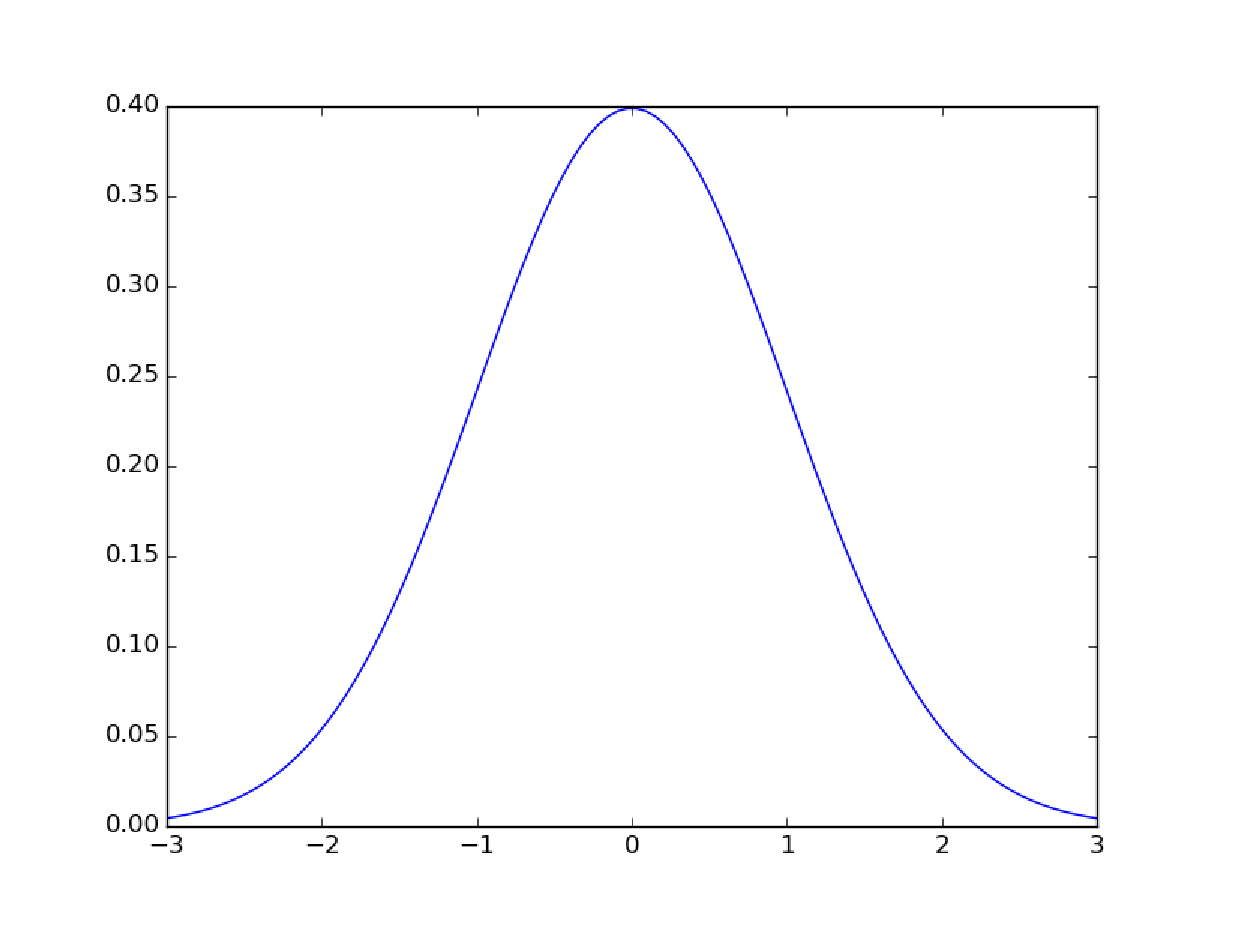
\includegraphics[width=0.5\linewidth]{figure_1}}
\caption{Стандартное нормальное распределение N(0,1)}
\label{ris:image}
\end{figure}
Перейдем к байесовской оценке:\\
Пусть $\theta \sim N(\theta_{\text{П}},\sigma_{\text{П}}^{2}) \to \theta_n^{*} = \frac{\frac{\theta_{\text{П}}}{\sigma_{\text{П}}^2} + \frac{\sum\limits_{i} x_i}{\sigma^2}}{\frac{1}{\sigma_{\text{П}}^2} + \frac{n}{\sigma^2}}, \theta_n^{*} \sim N(\frac{\frac{\theta_{\text{П}}}{\sigma_{\text{П}}^2} + \frac{n\theta_0}{\sigma^2}}{\frac{1}{\sigma_{\text{П}}^2} + \frac{n}{\sigma^2}},\frac{n\sigma^2}{(\frac{\sigma^2}{\sigma_{\text{П}}^2} + n)^2})$\\
$(\theta_0 - \hat{\theta_n^{*}}) \sim N(\frac{\frac{1}{\sigma_{\text{П}}^2}(\theta_{\text{П}} - \theta_0)}{\frac{1}{\sigma_{\text{П}}^2} + \frac{n}{\sigma^2}}, \frac{n\sigma^2}{(\frac{\sigma^2}{\sigma_{\text{П}}^2} + n)^2}) \sim N(\frac{(\theta_{\text{П}} - \theta_0)}{1 + \frac{n \sigma_{\text{П}}^2}{\sigma^2}}, \frac{n\sigma^2}{(\frac{\sigma^2}{\sigma_{\text{П}}^2} + n)^2}).$\\
Т.к. $\theta_0 \sim N(\theta_{\text{П}}, \sigma_{\text{П}}^2) \to$\\
$(\theta_0 - \hat{\theta_n^{*}}) \sim N(0, \frac{n\sigma^2}{(\frac{\sigma^2}{\sigma_{\text{П}}^2} + n)^2} + \frac{\sigma_{\text{П}}^2}{(1 + \frac{n\sigma_{\text{П}}^2}{\sigma^2})^2})$\\
Следовательно,\\
$\sqrt{n}(\theta_0 - \hat{\theta_n^{*}}) \sim N(0, \frac{n^2\sigma^2}{(\frac{\sigma^2}{\sigma_{\text{П}}^2} + n)^2} + \frac{n\sigma_{\text{П}}^2}{(1 + \frac{n\sigma_{\text{П}}^2}{\sigma^2})^2}) \sim N(0, \frac{n^2\sigma^2 + \frac{n\sigma^4}{\sigma_{\text{П}}^2}}{(\frac{\sigma^2}{\sigma_{\text{П}}^2} + n)^2}) \sim N(0, \frac{n\sigma^2}{(\frac{\sigma^2}{\sigma_{\text{П}}^2} + n)}) \sim N(0, \frac{\sigma^2}{\frac{\sigma^2}{n\sigma_{П}^2} + 1})$.\\
Следовательно, для байесовской оценки мы получаем нормально распределенную случайную величину, с мат.ожиданием, равным нулю и дисперсией $\frac{\sigma^2}{\frac{\sigma^2}{n\sigma_{\text{П}}^2} + 1};$\\
Возьмем $\sigma = 1, \sigma_{\text{П}} = \frac{1}{2}:$

\begin{figure}[h]
\center{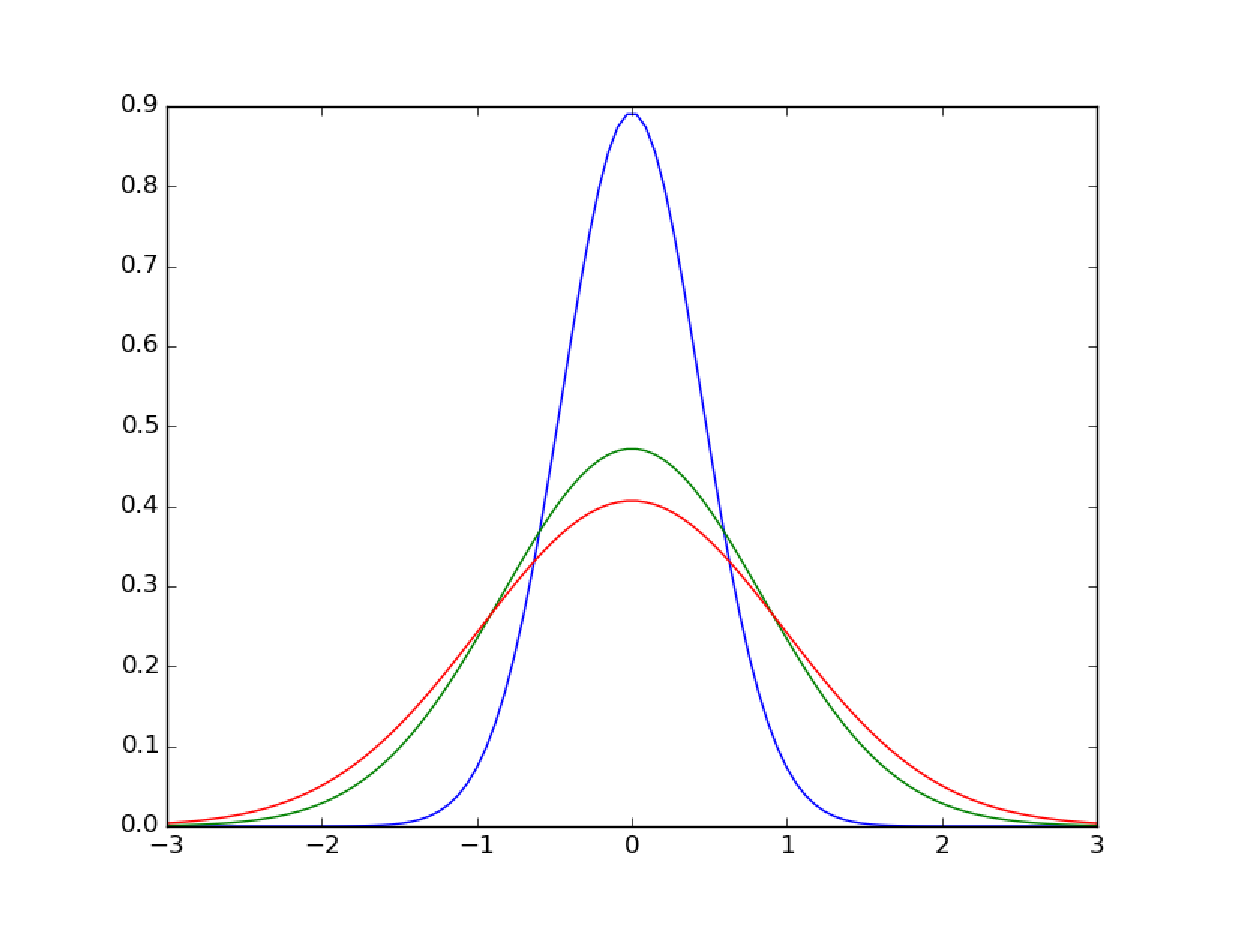
\includegraphics[width=0.5\linewidth]{figure_2}}
\caption{N(0,$\frac{1}{1 + \frac{4}{n}}$) при $n = 1, 10, 100$}
\label{ris:image}
\end{figure}

\end{document}